
The availability of powerful computing machines as well as widespread commercial tools allow for coping with engineering problems numerically. Numerical models aim at solving partial differential equations with applied initial and boundary conditions by transforming them into a discrete set of algebraic equations. The solution of those algebraic equations leads to an approximate result with respect to the initial PDE's~\cite{eth_introduction_to_finite_element}. The given process is summarised in Fig.~\ref{fig:computational_solution_technique}. 

\begin{figure}[H]
    \renewcommand{\baselinestretch}{0.7} 
    \centering
    \begin{tikzpicture}[node distance = 1.5cm, auto]
        \tikzstyle{decision} = [diamond, draw, fill=blue!20, text width=3cm, text badly centered, node distance=2.5cm, inner sep=0pt, scale=0.8]
        \tikzstyle{block} = [rectangle, draw, fill=blue!20, text width=4.5cm, text centered, rounded corners, node distance=6.0cm, scale=0.8, minimum height=0.5cm]
        \tikzstyle{line} = [draw, -latex']
        \tikzstyle{cloud} = [draw, ellipse,fill=red!20, node distance=3.0cm, minimum height=2em, scale=0.8]
  
    \node [block] (block1) {Proposal of partial differential equations (PDE's) with BC's and IC's};
    \node [block, right of=block1] (block2) {System of algebraic equations};
    \node [block, right of=block2] (block3) {Approximate solution};
    
    \path [line] (block1) -- (block2);
    \path [line] (block2) -- (block3);
    
    \draw [dashed, thin, black, ->] (2.35, 1.5) -- (2.35, 0);
    \draw [dashed, thin, black, ->] (7.1, 1.5) -- (7.1, 0);
    
    \node [draw, ellipse,fill=red!20, minimum height=2em, scale=0.8] at (2.35, 1.5) {Discretisation};
    \node [draw, ellipse,fill=red!20, minimum height=2em, scale=0.8] at (7.1, 1.5) {Equation solver};

    \end{tikzpicture}
    \caption{Schematic of the computational solution technique~\cite{eth_introduction_to_finite_element}.}
    \label{fig:computational_solution_technique}
\end{figure}

Numerical methods have several important advantages. First of all, they allow for finding an approximate solution of a real geometry rather than an exact result of a simplified shape, being the case of analytical analyses. In engineering applications, a numerical analysis serves for parameterising a given technical problem. Therefore, important design factors that influence operating conditions of a developed machine may be found and improved. The numerical approach gives answers to so called "what if" questions within a fast iterative thinking process~\cite{heat_transfer_practical_approach_cengel}. There are various numerical methods that serve for conversion of PDE's into a set of algebraic equations such as: 
\begin{itemize}
    \item Finite difference method.
    \item Finite element method.
    \item Finite volume method.
    \item Spectral method.
\end{itemize}

In this thesis, the finite element method (FEM) is covered. It is suitable for solving mechanical problems as well as the ones characterised by complex geometries, being a case of superconducting magnets. Many commercial numerical tools such as ANSYS or COMSOL use this method because of its capability to solve a large variety of physical problems. 

\subsection{Finite Element Method in Heat Conduction Problems}

This section gives an overview on consecutive steps applied while solving a heat conduction problem by means of a Finite Element Method. It is based on the the introductory course for FEM Modelling at ETH Zurich~\cite{eth_introduction_to_finite_element}. One can refer to this position to understand this topic in more details. Let's consider a partial differential equation of an unsteady one-dimensional heat conduction equation as 
\begin{equation}
    \frac{\partial T}{\partial t} = \frac{\partial}{\partial x} \left(k(x) \frac{\partial T}{\partial x} \right) + s(x), 
    \label{eqn:heat_conduction_pde}
\end{equation}
where $k(x)$ -- thermal conductivity as a function of space, $s(x)$ -- external heat source as a function of spaces. A temperature distribution is searched over the space and time, $T(x, t)$ that satisfies the given formula over the domain $\Omega \in \left[ 0, L \right]$. Two types of boundary conditions can be specified in the following problem: 
\begin{enumerate}
    \item 
    Dirichlet condition as \begin{equation}
    \left\{ \begin{array}{ lll }
    T(x_\text{A}, t) = T_\text{A},  \\ \\
    T(x_\text{B}, t) = T_\text{B},
    \end{array} \right.
    \end{equation}
    where $T_\text{A}$, $T_\text{B}$ -- constant temperatures at points A and B.
    
    \item Neumann condition as 
    \begin{equation}
    \left\{ \begin{array}{ lll }
    \left. k \frac{\partial T}{\partial x} \right|_{x=x_{\text{A},t}} = q_\text{A}, \\ \\
    \left. k \frac{\partial T}{\partial x} \right|_{x=x_{\text{B},t}} = q_\text{B},
    \end{array} \right.
    \label{eqn:neumann_bcs}
    \end{equation}
    where $q_\text{A}$ and $q_\text{A}$ heat flux at point A and B.
\end{enumerate}

In order to solve the equation being a function of time, the initial condition should be specified over the space as 
\begin{equation}
    T(x, t=0) = T_0(x).
\end{equation}

Discretisation involves a division of the analysed space into a finite number of elements consisting of nodes. Fig.~\ref{fig:1d_element} shows a one-dimensional element with two nodes at its extremities. 

\begin{figure}[H]
    \centering
    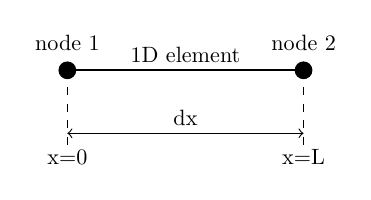
\begin{tikzpicture}[scale = 1]
        \filldraw[black] (0, 0) circle (3pt);
        \filldraw[black] (3, 0) circle (3pt);
        \draw[thick, black] (0, 0) -- (3, 0);
        \draw[thin, black, <->] (0, -0.8) -- (3, -0.8);
        \draw[thin, black, dashed] (0, 0) -- (0, -1);
        \draw[thin, black, dashed] (3, 0) -- (3, -1);
        \node[scale = 0.8] at (1.5, -0.6) {dx};
        \node[scale = 0.8] at (1.5, 0.2) {1D element};
        \node[scale = 0.8] at (0, 0.35) {node 1};
        \node[scale = 0.8] at (3, 0.35) {node 2};
        \node[scale = 0.8] at (0, -1.1) {x=0};
        \node[scale = 0.8] at (3, -1.1) {x=L};
    \end{tikzpicture}
    \caption{Exemplary one-dimensional 2-node element~\cite{eth_introduction_to_finite_element}.}
    \label{fig:1d_element}
\end{figure}

The more nodes is used in the element, the higher accuracy is obtained. However, the computing time increases as well. If two nodes are used for a 1D element, the temperature between them is interpolated linearly. The temperature over the longitudinal space is represented as
\begin{equation}
    T(x) \approx    
    \begin{bmatrix}  
    N_1(x) & N_2(x)    
    \end{bmatrix} 
    \begin{bmatrix}  
    T_1(x) \\  T_2(x) 
    \end{bmatrix} 
    = \vect{N} \vect{X}, 
    \label{eqn:linear_shape_function}
\end{equation}
where $N_1(x)$ and $N_2(x)$ -- the linear shape functions that allow for approximating the temperature over the continuous space. The shape functions can be reformulated as 
\begin{equation}
    \left\{ \begin{array}{ lll }
    N_1(x) = 1 - \frac{x}{L} \\ \\
    N_2(x) = \frac{x}{L},
    \end{array} \right.
    \label{eqn:shape_functions_representation}
\end{equation}
where $L$ -- length between two nodes in Fig.\ref{fig:1d_element}, $x$ -- spatial variable varying for $x \in [0, L]$. The shape functions are illustrated in Fig.~\ref{fig:linear_shape_functions}.

\begin{figure}[H]
    \centering
    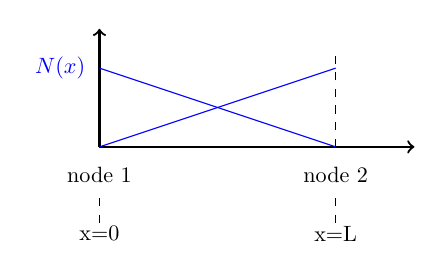
\begin{tikzpicture}[scale = 1]
    
        \draw[thick, black, ->] (0, 0) -- (4, 0);
        \draw[thick, black, ->] (0, 0) -- (0, 1.5);
        
        \draw[blue] (0, 0) -- (3, 1);
        \draw[blue] (0, 1) -- (3, 0);
        \node[scale = 0.8, blue] at (-0.5, 1) {$N(x)$};
        
        \draw[thin, black, dashed] (0, -0.65) -- (0, -1);
        \draw[thin, black, dashed] (3, -0.65) -- (3, -1);
        \draw[very thin, black, dashed] (3, 0) -- (3, 1.25);
    
        \node[scale = 0.8] at (0, -0.35) {node 1};
        \node[scale = 0.8] at (3, -0.35) {node 2};
        
        \node[scale = 0.8] at (0, -1.1) {x=0};
        \node[scale = 0.8] at (3, -1.1) {x=L};
    
    \end{tikzpicture}
    \caption{Representation of linear shape functions $N(x)$~\cite{eth_introduction_to_finite_element}.}
    \label{fig:linear_shape_functions}
\end{figure}

After substituting the approximated temperature distribution from (\ref{eqn:linear_shape_function}) to the differential equation from (\ref{eqn:heat_conduction_pde}), one obtains

\begin{equation}
     \frac{\partial}{\partial t} \left(   
     \begin{bmatrix}  
     N_1(x) & N_2(x)    
    \end{bmatrix} 
    \begin{bmatrix}  
    T_1(x) \\  T_2(x) 
    \end{bmatrix} \right) 
    - \frac{\partial}{\partial x} \left( k(x) \frac{\partial}{\partial x} \left( 
    \begin{bmatrix}  
    N_1(x) & N_2(x)    
    \end{bmatrix} 
    \begin{bmatrix}  
    T_1(x) \\  T_2(x) 
    \end{bmatrix} \right) \right) - s(x) = R,
    \label{eqn:residual_function}
\end{equation}
where $R$ -- a residual error being a result of the discretisation process. In the continuous solution, the residual is equal to zero. Equation~(\ref{eqn:residual_function}) still cannot be solved because the number of variables exceeds the number of equations. In order to solve this problem, Equation~(\ref{eqn:residual_function}) is multiplied by a set of so called "weighting functions". The weighted residual of such an expression must be equal to zero. One of the method, proposing a specific weighting function is called a Galerkin method. It is more explained in~\cite[p.~1-11]{eth_introduction_to_finite_element}.

In the next steps, the analysis is simplified by assuming the thermal conductivity and heat source independent of space. After applying the weighting functions, a set of algebraic equations is obtained as 

\begin{equation}
    \begin{bmatrix}  
    \frac{L}{3} & \frac{L}{6} \\
    \frac{L}{6} & \frac{L}{3}
    \end{bmatrix} 
    \begin{bmatrix}  
    \frac{\partial T_1}{\partial t} \\
    \frac{\partial T_2}{\partial t}
    \end{bmatrix} 
    + \bar k
    \begin{bmatrix}  
    \frac{1}{L} & -\frac{1}{L} \\
    -\frac{1}{L} & \frac{1}{L}
    \end{bmatrix} 
    \begin{bmatrix}  
    T_1 \\
    T_2
    \end{bmatrix} 
    = 
    \begin{bmatrix}  
    N_1 \left. q_\text{A} \right|_{x_\text{A}} \\
    N_2 \left. q_\text{A} \right|_{x_\text{A}}
    \end{bmatrix} 
    + \bar s 
    \begin{bmatrix}  
    \frac{L}{2} \\
    \frac{L}{2}
    \end{bmatrix},
    \label{eqn:set_algebraic_equations}
\end{equation}
where $\bar k$ -- constant thermal conductivity over each volume element $\left[x_\text{A}, x_\text{B} \right]$,  $\bar s$ -- constant heat source over the same element volume, $q_\text{A}$ -- heat flux at point A, $q_\text{B}$ -- heat flux at point B. In the derivation process, Neumann boundary conditions were assumed, as shown in~(\ref{eqn:neumann_bcs}). Equation~(\ref{eqn:set_algebraic_equations}) can be written in a matrix form as

\begin{equation}
    \vect{A} \frac{\partial \vect{T}}{\partial t} + \vect{B} \vect{T} = \vect{F},
\end{equation}
where 

\begin{equation}
    \vect{A} = 
    \begin{bmatrix}  
    \frac{L}{3} & \frac{L}{6} \\
    \frac{L}{6} & \frac{L}{3}
    \end{bmatrix},
\end{equation}

\begin{equation}
    \vect{B} = 
    \begin{bmatrix}  
    \frac{1}{L} & -\frac{1}{L} \\
    -\frac{1}{L} & \frac{1}{L}
    \end{bmatrix},
\end{equation}

\begin{equation}
    \vect{T} = 
    \begin{bmatrix}  
    T_1 \\
    T_2
    \end{bmatrix},
\end{equation}

\begin{equation}
    \vect{F} = 
    \begin{bmatrix}  
    N_1 \left. q_\text{A} \right|_{x_\text{A}} \\
    N_2 \left. q_\text{A} \right|_{x_\text{A}}
    \end{bmatrix} 
    + \bar s 
    \begin{bmatrix}  
    \frac{L}{2} \\
    \frac{L}{2}
    \end{bmatrix}.
\end{equation}

Since the problem is transient, one should discretise the temperature time derivative. A~finite difference method is used with an implicit discretisation as

\begin{equation}
    \vect{A} \frac{\vect{T}^{n+1} - \vect{T}^n}{\Delta t} + \vect{B} \vect{T}^{n+1} = \vect{F},
\end{equation}
where $\Delta t$ -- a time step between two iterations of the solution, $\vect{T}^n$ -- known temperature vector from the current iteration, $\vect{T}^{n+1}$ -- unknown temperature vector from the next iteration to compute. After rearranging the formula, one obtains
\begin{equation}
    \vect{K} \vect{T}^{n+1} =\vect{M} \vect{T}^{n} + \vect{F},
\end{equation}
where 
\begin{equation}
    \vect{K} = \frac{1}{\Delta t} \vect{A} + \vect{B},
\end{equation}

\begin{equation}
    \vect{M} = \frac{1}{\Delta t} \vect{A}.
\end{equation}

The matrix $\vect{K}$ is called the element stiffness matrix. While conducting a simulation with more degrees of freedom (DOF), i.e higher number of nodes, the stiffness matrices of every single element add up to form a large global stiffness matrix. The more DOF's are used, the more time consuming the problem becomes.

\subsection{Quench Modelling in Superconducting Magnets}

A quench is a multi-physics problem including thermal, electric and magnetic phenomena. In each of these events, one copes with non-linearities of material properties mainly due to a wide range of temperatures at which a magnet operates. From a~design standpoint, a superconducting magnet should sustain a~temperature varying from a~cryogenic one up to the thermal failure limit of an~insulation layer usually remaining in the~limit of a~room temperature. In the given range, a quench simulation meets the following difficulties: 

\begin{enumerate}
    \item Non-linear heat capacity and thermal conductivity of magnet materials. They are a function of temperature and, in some cases, -- a~magnetic field. 
    \item Non-linear resistivity of copper being a function of temperature and a magnetic field.
    \item Non-linear inductance of a superconducting magnet due to the influence of an iron yoke. 
    \item The influence of eddy currents that may cause a quench back during the discharge of a magnet.
    \item Non-linear thermal and fluid-dynamic properties of a cooling helium used in superconducting magnets. They should be taken into consideration while analysing the exchange of heat between the liquid medium and a quenching coil. 
\end{enumerate}

Apart from a multi-physics environment that requires a coupling of several simulations altogether, the complexity of a quench analysis is also due to the following reasons: 
\begin{enumerate}
    \item Multi-rate problem -- thermal and electrical time constants in transient analyses may vary by several orders of magnitude.
    \item Multi-domain problem -- different materials interact with each other, being in some cases also at a varying solid or liquid state if helium is considered.
    \item Multi-scale problem -- analysis of components with extremely different sizes may be considered varying from a 10~$\upmu$m-wide filament in a strand to a~10~m-long magnet as a whole.
\end{enumerate}

As presented in Fig.~\ref{fig:magnet_design_domains}, the magnet design is an iterative process in which four main studies ought to be conducted: electromagnetic, mechanical as well as the ones related to the quench protection and to the circuit. The change of a design parameter in one element entails the correction of different one in another constituent. As an example, a study for the quench protection includes the verification whether the magnet does not overheat during the discharge. If the analysis proves a wrong design, the information comes back to electromagnetic studies in which a new design of a coil has to be carried out~\cite{quench_protection_system_applied_prioli}.

\begin{figure}[H]
    \centering
    \begin{tikzpicture}
    \node at (0,0) {\includegraphics[width=.45\textwidth]{sections/introduction/figures/domains_design_magnet.png}};
    \end{tikzpicture}
    \caption{Domain considered during the design process of a superconducting magnets~\cite{quench_protection_system_applied_prioli}.}
    \label{fig:magnet_design_domains}
\end{figure}

Fig.~\ref{fig:model_complexity_vs_completeness} shows a thermal analysis workflow with respect to the problem complexity from a quench protection perspective. On one hand, the most accurate thermal map of a magnet is desired which allows for lowering the design safety coefficients. However, in order to obtain the least approximate solution, the number of degrees needs to be increased by applying a denser mesh or an additional dimension in the simulation. The more complete model is created, the longer iteration loops between different studies from Fig~\ref{fig:magnet_design_domains} become. In fact, they should be short in order to enable multiple design teams for a fast exchange of information. Thus, the modelling approach in a quench protection study is a compromise between the model completeness and the computation time.

\begin{figure}[H]
  \centering
  \begin{tikzpicture}
      \begin{polaraxis}
      [
      axis line style = {draw=none}, 
      hide y axis,
      hide x axis,
      no marks,
      samples=201,
      smooth,
      domain=0:2
      ]
      \addplot+ (4*180*x,x);
    \end{polaraxis}
    
    \node[black, scale=0.72] at (3.5,3.2) {0D};
    \node[black, scale=0.72] at (3.5,3.9) {1D};
    \node[black, scale=0.728] at (3.5,2.6) {2D network};
    \node[black, scale=0.72] at (3.5,4.7) {2D FEM};
    \node[black, scale=0.72] at (3.5,1.75) {3D Analytical};
    \node[black, scale=0.72] at (3.3,5.4) {3D FEM + Analytical};
    \node[black, scale=0.72] at (3.35,0.9) {3D FEM};
    \node[black, scale=0.72, text width=2.2cm] at (6.9,3.9) {Model \\ completeness};
    
    \draw[black, ->] (9,1) -- (14,1);
    \draw[black, ->] (9,1) -- (9,4.5);
    \draw[blue] (9,1) .. controls +(10:1cm) and +(-135:1cm) .. (12,2);
    \draw[blue] (12,2) .. controls +(45:1cm) and +(-100:1cm) .. (13,4);
    \node[black, scale=0.72] at (13,0.7) {Model completeness};
    \node[black, scale=0.72, text width=2.3cm] at (10,4.2) {Computation \\ time};
  \end{tikzpicture}
  \caption{Left: thermal analysis workflow with respect to the problem complexity; Right: computation time vs. model complexity~\cite{steam_architecture_presentation}.}
  \label{fig:model_complexity_vs_completeness}
\end{figure}



























% In a FEM method, Equation~(\ref{eqn:residual_function}) is multiplied by a set of so called "weighting functions". The weighted residual of such an expression must be equal to zero. Various methods propose different weighting functions. In this section, a Galerkin method is explained which is also described in~\cite{eth_introduction_to_finite_element}. The weighting functions are identical to the shape functions in this approach. Therefore, Equation~(\ref{eqn:residual_function}) is multiplied by a weighting function matrix composed of the shape functions~$N$. Then, the formula is integrated over the volume of an element as 

% \begin{equation}
% \begin{split}
%          & \int_{0}^{L} 
%          \begin{bmatrix}  
%          N_1 \\ N_2   
%         \end{bmatrix} 
%          \frac{\partial}{\partial t} \left(   
%          \begin{bmatrix}  
%          N_1 & N_2   
%         \end{bmatrix} 
%         \begin{bmatrix}  
%         T_1 \\  T_2 
%         \end{bmatrix} \right) dx -
%         \\
%         & - \int_{0}^{L} 
%         \begin{bmatrix}  
%          N_1 \\ N_2   
%         \end{bmatrix}
%         \frac{\partial}{\partial x} \left( k(x) \frac{\partial}{\partial x} \left( 
%         \begin{bmatrix}  
%         N_1 & N_2    
%         \end{bmatrix} 
%         \begin{bmatrix}  
%         T_1 \\  T_2 
%         \end{bmatrix} \right) \right) dx
%         - \int_{0}^{L} 
%         \begin{bmatrix}  
%          N_1 \\ N_2   
%         \end{bmatrix}
%         s(x) dx
%         = 
%         \begin{bmatrix}  
%          0 \\ 0 
%         \end{bmatrix}.
%         \label{eqn:weighting_functions_fem}
% \end{split}
% \end{equation}


% By applying the Green's theorem to the given equation, one obtains a one-dimensional solution for $\Omega = \left[x_\text{A}, x_\text{B} \right]$ as
% \begin{equation}
%     \int_{\Omega}^{} N_\text{i} \frac{\partial}{\partial x} \left( k(x) \frac{\partial N_\text{j}}{\partial x} \right) dx = - \int_{\Omega} k(x) \frac{\partial N_\text{i}}{\partial x} \frac{\partial N_\text{j}}{\partial x} dx + \left. k(x) N_\text{i} \frac{\partial N_\text{j}}{\partial x} \right|^{x_\text{B}}_{x_\text{A}}.
%     \label{eqn:greens_theorem_fem}
% \end{equation}

% Let the heat source and thermal conductivity be constant over space and denoted as $\bar s$ and $\bar k$. Using Equation~(\ref{eqn:greens_theorem_fem}), the Equation~(\ref{eqn:weighting_functions_fem}) can be rewritten into

% \begin{equation}
%     \begin{split}
%     \begin{bmatrix}  
%     \int_0^L N_1 N_1 dx & \int_0^L N_1 N_2 dx \\
%     \int_0^L N_2 N_1 dx & \int_0^L N_2 N_2 dx
%     \end{bmatrix}
%     \frac{\partial}{\partial t}
%     \begin{bmatrix}  
%         T_1 \\  T_2 
%     \end{bmatrix}
%     + \bar k
%     \begin{bmatrix}  
%     \int_0^L \frac{N_1}{\partial x} \frac{N_1}{\partial x} dx & \int_0^L \frac{N_1}{\partial x} \frac{N_2}{\partial x} dx \\
%     \int_0^L \frac{N_2}{\partial x} \frac{N_1}{\partial x} dx & 
%     \int_0^L \frac{N_2}{\partial x} \frac{N_2}{\partial x} dx
%     \end{bmatrix}
%     \begin{bmatrix}  
%         T_1 \\  T_2 
%     \end{bmatrix} = \\
%     = \bar s 
%     \begin{bmatrix}  
%         \int_0^L N_1 dx \\ \int_0^L N_2 dx
%     \end{bmatrix}
%     + 
%     \begin{bmatrix}  
%         \left. N_1 q_\text{A} \right|_{x_\text{A}} \\ \left. N_2 q_\text{B} \right|_{x_\text{B}}
%     \end{bmatrix}
%     \end{split}.
% \end{equation}

% By using the shape functions specified in~(\ref{eqn:shape_functions_representation}), an algebraic equation is obtained as

% \begin{equation}
%     \begin{bmatrix}  
%     \frac{L}{3} & \frac{L}{6} \\
%     \frac{L}{6} & \frac{L}{3}
%     \end{bmatrix} 
%     \begin{bmatrix}  
%     \frac{\partial T_1}{\partial t} \\
%     \frac{\partial T_2}{\partial t}
%     \end{bmatrix} 
%     + \bar k
%     \begin{bmatrix}  
%     \frac{1}{L} & -\frac{1}{L} \\
%     -\frac{1}{L} & \frac{1}{L}
%     \end{bmatrix} 
%     \begin{bmatrix}  
%     T_1 \\
%     T_2
%     \end{bmatrix} 
%     = 
%     \begin{bmatrix}  
%     N_1 \left. q_\text{A} \right|_{x_\text{A}} \\
%     N_2 \left. q_\text{A} \right|_{x_\text{A}}
%     \end{bmatrix} 
%     + \bar s 
%     \begin{bmatrix}  
%     \frac{L}{2} \\
%     \frac{L}{2}
%     \end{bmatrix} 
% \end{equation}

% In this case, the number of equations corresponds to the number of unknowns, $T_1$ and $T_2$. 

% \subsubsection{Equation Solver, Approximate Solution}

% \begin{equation}
%     \vect{M} \frac{\partial \vect{T}}{\partial t} + \vect{K} \vect{T} = \vect{F}
% \end{equation}

% \begin{equation}
%     \vect{M} \frac{\vect{T}^{n+1} - \vect{T}^n}{\Delta t} + \vect{K} \vect{T}^{n+1} = \vect{F}
% \end{equation}

% Rearranging 
% \begin{equation}
%     \left( \frac{1}{\Delta t} \vect{M} + \vect{K} \right) \vect{T}^{n+1} = \frac{1}{\Delta t} \vect{M} \vect{T}^{n} + \vect{F}
% \end{equation}
